% The quantized element matrix in difference form with a scale per node pair: the off-diagonal
% node blocks K_pq, p < q, as int8 codes, an 8-bit factor per pair and a scale per element.
\documentclass[border=2pt]{standalone}
% Shared preamble of the format diagrams: colours of the paper's figures (paper_figures.py) and
% the drawing styles.  Each diagram is a standalone document built to a PDF of the text width.
\usepackage{amsmath,amssymb}
\usepackage{tikz}
\usetikzlibrary{arrows.meta,calc,decorations.pathreplacing,patterns,positioning}

\definecolor{cindex}{HTML}{BDBDBD}  % column indices, offsets, row pointers
\definecolor{cvalue}{HTML}{6E6E6E}  % floating-point values (BSR)
\definecolor{cpoint}{HTML}{1B9E77}  % quadrature-point store
\definecolor{celem}{HTML}{1F78B4}   % element matrix
\definecolor{cqbsr}{HTML}{A6761D}   % quantized BSR
\definecolor{cscale}{HTML}{E6AB02}  % scales
\definecolor{cmean}{HTML}{7570B3}   % f32 element mean

\tikzset{
  >={Stealth[length=4pt]},
  grid/.style={draw=black!45, line width=0.25pt},
  frame/.style={draw=black!70, line width=0.5pt},
  title/.style={font=\small\bfseries, anchor=west, inner sep=0pt},
  lab/.style={font=\footnotesize, inner sep=1pt},
  note/.style={font=\scriptsize, text=black!75, inner sep=1pt, execute at begin node={\hyphenpenalty=10000\exhyphenpenalty=10000}},
  num/.style={font=\tiny, inner sep=0pt},
  brace/.style={decorate, decoration={brace, amplitude=3pt, raise=1pt}, line width=0.4pt},
  arr/.style={->, line width=0.5pt, black!70},
  pad/.style={pattern=north east lines, pattern color=black!30},
}

% \cell{x}{y}{w}{h}{fill}: a filled rectangle with a thin outline, lower-left corner at (x,y).
\newcommand{\cell}[5]{\filldraw[fill=#5, grid] (#1,#2) rectangle ++(#3,#4);}
% \blk{x}{y}{s}{fill}: a 3x3 block of side s with its 3x3 entry grid.
\newcommand{\blk}[4]{%
  \filldraw[fill=#4, grid] (#1,#2) rectangle ++(#3,#3);
  \draw[draw=white, line width=0.25pt] (#1,#2) ++(#3/3,0) -- ++(0,#3) ++(#3/3,0) -- ++(0,-#3);
  \draw[draw=white, line width=0.25pt] (#1,#2) ++(0,#3/3) -- ++(#3,0) ++(0,#3/3) -- ++(-#3,0);
  \draw[grid] (#1,#2) rectangle ++(#3,#3);}
% \vthree{x}{y}{fill}: a 3-vector (one node's components) as three small cells, left end at (x,y).
\newcommand{\vthree}[3]{\foreach \k in {0,1,2} \filldraw[fill=#3, grid] (#1+\k*0.14,#2) rectangle ++(0.14,0.14);}
% \op{x}{y}{symbol}: an operation in a small circle.
\newcommand{\op}[3]{\node[circle, draw=black!70, line width=0.4pt, inner sep=0.5pt, minimum size=9pt, font=\tiny] at (#1,#2) {#3};}

\begin{document}
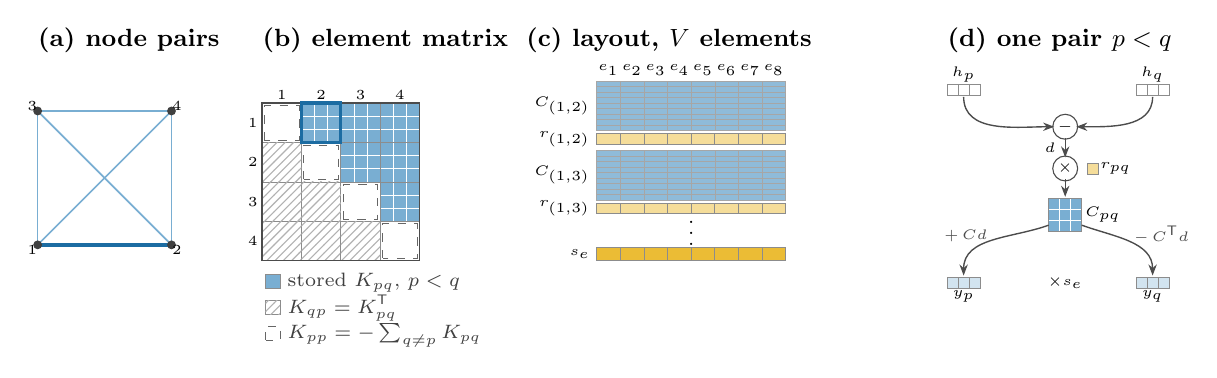
\begin{tikzpicture}
  % ---------------------------------------------------------------- (a) node pairs
  \node[title] at (0, 3.35) {(a) node pairs};
  \coordinate (n1) at (0,0.75); \coordinate (n2) at (1.7,0.75);
  \coordinate (n3) at (0,2.45); \coordinate (n4) at (1.7,2.45);
  \foreach \a/\b in {n1/n2, n1/n3, n1/n4, n2/n3, n2/n4, n3/n4} \draw[celem!60, line width=0.6pt] (\a) -- (\b);
  \draw[celem!90!black, line width=1.6pt] (n1) -- (n2);
  \foreach \n/\pos in {1/below left, 2/below right, 3/above left, 4/above right} {
    \fill[black!75] (n\n) circle (1.6pt);
    \node[num, \pos] at (n\n) {$\n$};
  }

  % ---------------------------------------------------------------- (b) which blocks are stored
  \begin{scope}[shift={(2.85,0.55)}]
    \def\s{0.5}
    \node[title] at (0, 2.8) {(b) element matrix};
    \foreach \p in {1,...,4} \foreach \q in {1,...,4} {
      \pgfmathsetmacro{\x}{(\q-1)*\s}\pgfmathsetmacro{\y}{(4-\p)*\s}
      \ifnum\p<\q \blk{\x}{\y}{\s}{celem!60}\fi
      \ifnum\p>\q \filldraw[fill=white, grid] (\x,\y) rectangle ++(\s,\s); \fill[pad] (\x,\y) rectangle ++(\s,\s); \fi
      \ifnum\p=\q \draw[grid, dashed, draw=black!60] (\x+0.03,\y+0.03) rectangle ++(\s-0.06,\s-0.06); \fi
    }
    \foreach \p in {1,...,4} {
      \node[num, anchor=east] at (-0.05, {(4-\p)*\s+\s/2}) {$\p$};
      \node[num, anchor=south] at ({(\p-1)*\s+\s/2}, 4*\s+0.04) {$\p$};
    }
    \draw[frame] (0,0) rectangle (4*\s, 4*\s);
    \draw[celem!90!black, line width=1.2pt] (\s, 3*\s) rectangle ++(\s,\s);
    \node[note, anchor=north west, align=left] at (0, -0.12)
      {\tikz[baseline=0.2ex]\filldraw[fill=celem!60, grid] (0,0) rectangle (0.18,0.18); stored $K_{pq}$, $p<q$\\
       \tikz[baseline=0.2ex]{\filldraw[fill=white, grid] (0,0) rectangle (0.18,0.18); \fill[pad] (0,0) rectangle (0.18,0.18);} $K_{qp}=K_{pq}^{\mathsf T}$\\
       \tikz[baseline=0.2ex]\draw[grid, dashed, draw=black!60] (0,0) rectangle (0.18,0.18); $K_{pp}=-\sum_{q\ne p}K_{pq}$};
  \end{scope}

  % ---------------------------------------------------------------- (c) layout of a block
  \begin{scope}[shift={(7.1,0)}]
    \def\w{0.3}
    \node[title] at (-0.9, 3.35) {(c) layout, $V$ elements};
    \foreach \v in {1,...,8} \node[num, anchor=south] at ({(\v-0.5)*\w}, 2.9) {$e_{\v}$};
    % pair (1,2): 9 codes and its factor; pair (1,3); ...
    \def\rh{0.07}
    \foreach \pair/\y in {{(1,2)}/2.2, {(1,3)}/1.32} {
      \foreach \e in {0,...,8} \foreach \v in {0,...,7}
        \filldraw[fill=celem!50, draw=black!35, line width=0.15pt] (\v*\w, {\y+(8-\e)*\rh}) rectangle ++(\w, \rh);
      \foreach \v in {0,...,7} {\cell{\v*\w}{\y-0.17}{\w}{0.13}{cscale!40}}
      \node[num, anchor=east] at (-0.08, {\y+4.5*\rh}) {$C_{\pair}$};
      \node[num, anchor=east] at (-0.08, \y-0.105) {$r_{\pair}$};
    }
    \node[font=\scriptsize, inner sep=0pt] at (4*\w, 1.0) {$\vdots$};
    \foreach \v in {0,...,7} {\cell{\v*\w}{0.55}{\w}{0.17}{cscale!80}}
    \node[num, anchor=east] at (-0.08, 0.635) {$s_e$};
  \end{scope}

  % ---------------------------------------------------------------- (d) the application, one pair
  \begin{scope}[shift={(11.55,0)}]
    \node[title] at (0, 3.35) {(d) one pair $p<q$};
    % inputs
    \vthree{0.0}{2.65}{white} \node[num, anchor=south] at (0.21, 2.81) {$h_p$};
    \vthree{2.4}{2.65}{white} \node[num, anchor=south] at (2.61, 2.81) {$h_q$};
    \op{1.5}{2.25}{$-$}
    \draw[arr] (0.21, 2.63) to[out=-90, in=180] (1.36, 2.25);
    \draw[arr] (2.61, 2.63) to[out=-90, in=0] (1.64, 2.25);
    % the pair factor
    \op{1.5}{1.72}{$\times$}
    \draw[arr] (1.5, 2.11) -- (1.5, 1.86);
    \cell{1.78}{1.65}{0.14}{0.14}{cscale!40} \node[num, anchor=west] at (1.94, 1.72) {$r_{pq}$};
    \node[num, anchor=east] at (1.38, 1.98) {$d$};
    % the block
    \blk{1.29}{0.92}{0.42}{celem!60}
    \node[num, anchor=west] at (1.75, 1.13) {$C_{pq}$};
    \draw[arr] (1.5, 1.58) -- (1.5, 1.36);
    % outputs
    \vthree{0.0}{0.2}{celem!20} \node[num, anchor=north] at (0.21, 0.18) {$y_p$};
    \vthree{2.4}{0.2}{celem!20} \node[num, anchor=north] at (2.61, 0.18) {$y_q$};
    \draw[arr] (1.29, 1.0) to[out=200, in=90] node[num, above left, pos=0.55] {$+\,C d$} (0.21, 0.36);
    \draw[arr] (1.71, 1.0) to[out=-20, in=90] node[num, above right, pos=0.55] {$-\,C^{\mathsf T} d$} (2.61, 0.36);
    \node[num] at (1.5, 0.27) {$\times s_e$};
  \end{scope}
\end{tikzpicture}
\end{document}
